\bta{核反应核能}

\begin{enumerate}
	%\renewcommand{\labelenumi}{\arabic{enumi}.}
	% A(\Alph) a(\alph) I(\Roman) i(\roman) 1(\arabic)
	%设定全局标号series=example	%引用全局变量resume=example
	%[topsep=-0.3em,parsep=-0.3em,itemsep=-0.3em,partopsep=-0.3em]
	%可使用leftmargin调整列表环境左边的空白长度 [leftmargin=0em]
	\item
\exwhere{$ 2019 $ 年 $ 4 $ 月浙江物理选考}
静止在匀强磁场中的原子核  \ce{X}  发生$ \alpha $衰变后变成新原子核   \ce{Y} 。已知核
 \ce{X}  的质量数为  \ce{A} ,电荷数为  \ce{Z} ,核  \ce{X} 、核  \ce{Y}  和$ \alpha $粒子的质量分别为 $ m_{\mathnormal{X}} $、$ m_{\mathnormal{Y}} $和 $ m _{\alpha} $,$ \alpha $粒子在磁场中运
动的半径为 $ R $。则 \xzanswer{AC} 

\fourchoices
{衰变方程可表示为 \ce{_{Z}^{A}X \rightarrow ^{A-4}_{Z-2}Y + _{2}^{4}He}}
{核 \ce{Y} 的结合能为$\left(m_{\mathnormal{X}}-m_{\mathnormal{Y}}-m_{\alpha}\right) c^{2}$}
{核 \ce{Y} 在磁场中运动的半径为$\frac{2 R}{\mathnormal{Z}-2}$}
{核 \ce{Y} 的动能为$E_{K \mathnormal{Y}}=\frac{m_{Y}\left(m_{\mathnormal{X}}-m_{\mathnormal{Y}}-m_{\alpha}\right) c^{2}}{m_{\mathnormal{Y}}+m_{\alpha}}$}


\item 
\exwhere{$ 2019 $ 年物理全国\lmd{2}卷}
太阳内部核反应的主要模式之一是质子$ - $质子循坏,循环的结果可表示为
$4_{1}^{1} \mathrm{H} \rightarrow{ }_{2}^{4} \mathrm{He}+2{ }_{1}^{0} \mathrm{e}+2\nu$,已知 \ce{^{1}_{1}H} 和 \ce{^{4}_{2}He} 的质量分别为 $ m_{P}=1.0078 \ u $ 和 $ m_{ \alpha } =4.0026 \ u $,$ 1 \ u=931 \ MeV/c^{2} $,$ c $
为光速。在 $ 4 $ 个 \ce{^{1}_{1}H} 转变成 $ 1 $ 个 \ce{^{4}_{2}He} 的过程中,释放的能量约为 \xzanswer{C} 

\fourchoices
{$ 8 \ MeV $}
{$ 16 \ MeV $}
{$ 26 \ MeV $}
{$ 52 \ MeV $}




\item 
\exwhere{$ 2019 $ 年物理天津卷}
我国核聚变反应研究大科学装置“人造太阳”$ 2018 $ 年获得重大突破,等离子
体中心电子温度首次达到 $ 1 $ 亿度,为人类开发利用核聚变能源奠定了重要的技术基础。下列关于聚
变的说法正确的是 \xzanswer{AD} 
\begin{figure}[h!]
	\centering
	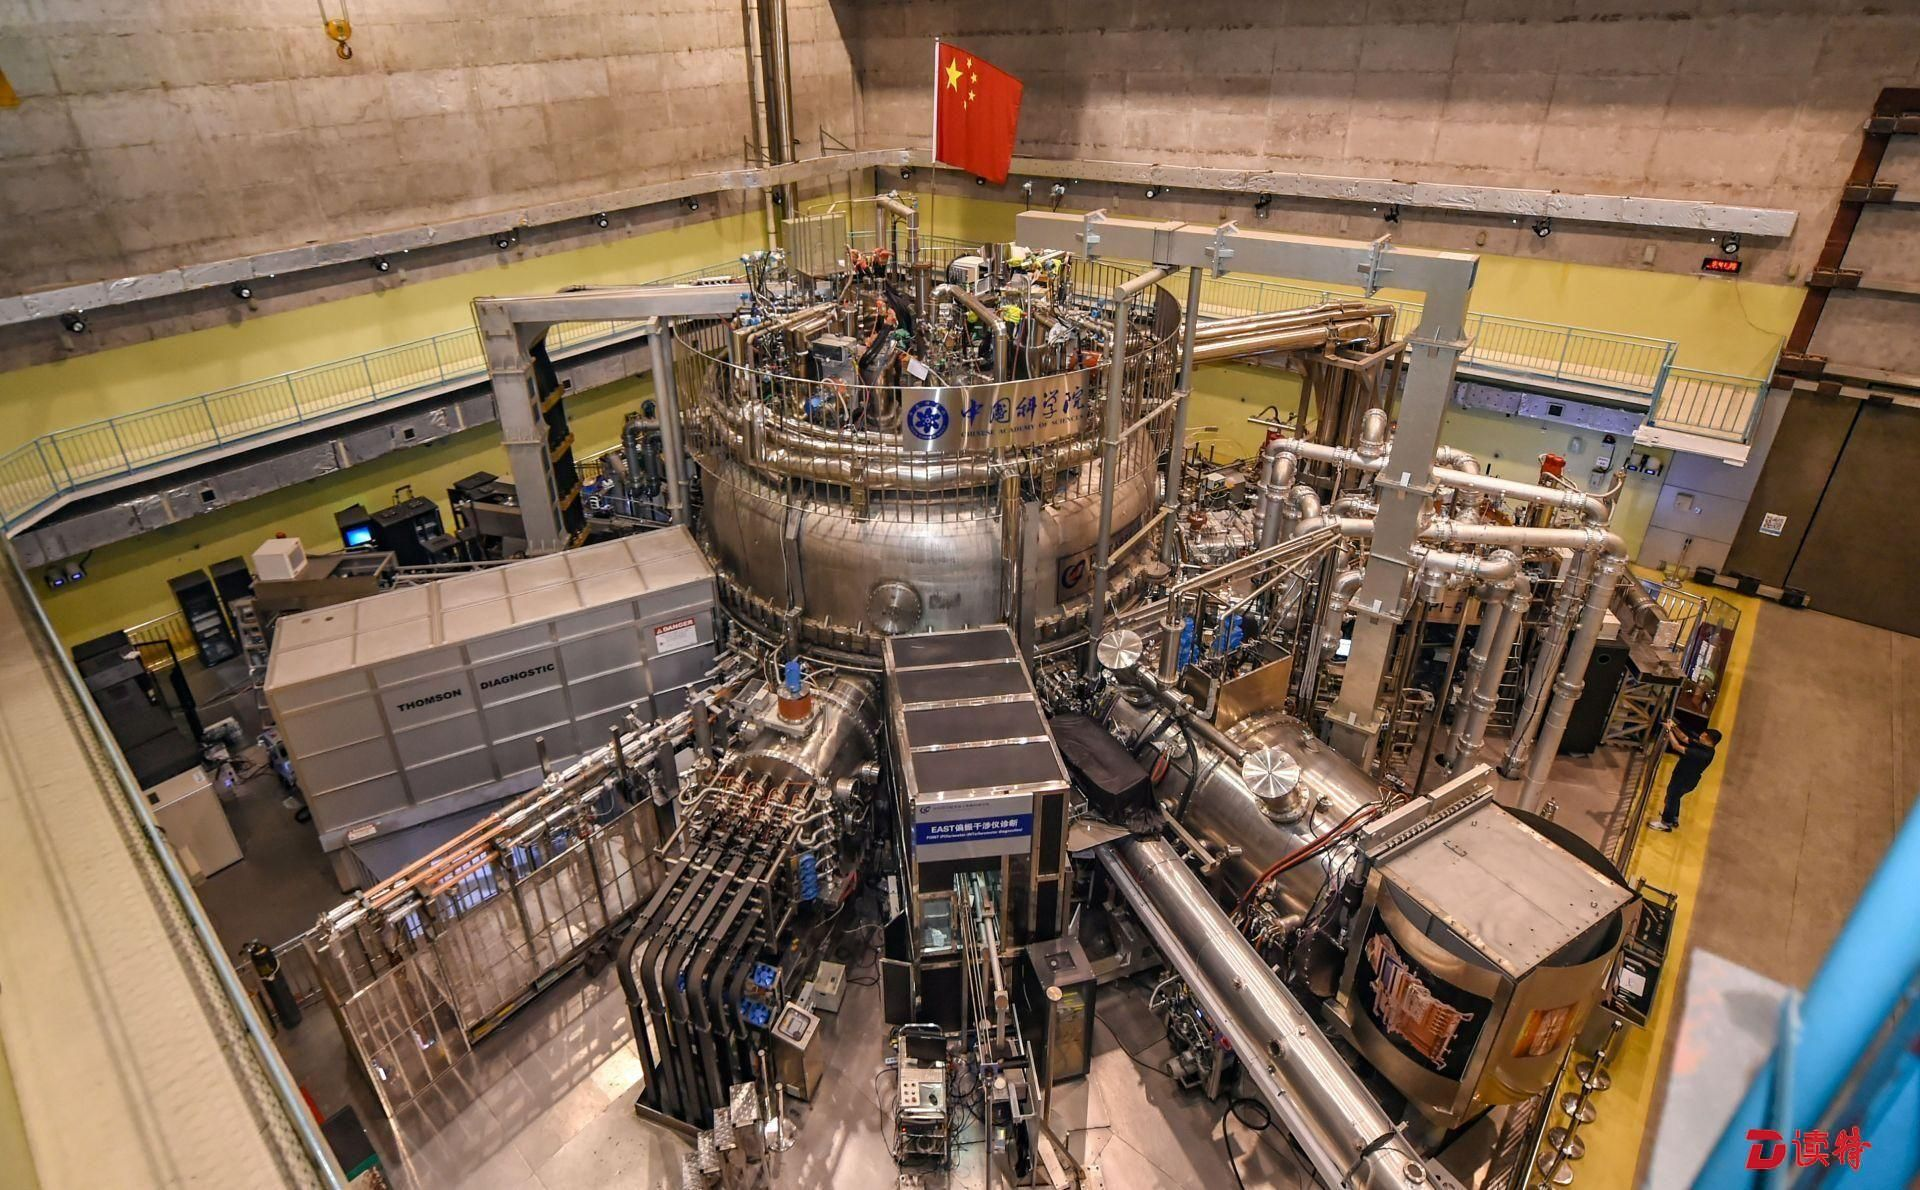
\includegraphics[width=0.3\linewidth]{picture/screenshot069.png}
\end{figure}



\fourchoices
{核聚变比核裂变更为安全、清洁}
{任何两个原子核都可以发生聚变}
{两个轻核结合成质量较大的核,总质量较聚变前增加}
{两个轻核结合成质量较大的核,核子的比结合能增加}



\item 
\exwhere{$ 2014 $ 年物理上海卷}
核反应方程 ${ }_{4}^{9} \mathrm{Be}+{ }_{2}^{4} \mathrm{He} \rightarrow{ }_{6}^{12} \mathrm{C}+\mathrm{X}$ 中的 $ \mathrm{X} $ 表示 \xzanswer{D} 

\fourchoices
{质子}
{电子}
{光子}
{中子}



\item 
\exwhere{$ 2013 $ 年上海卷}
放射性元素 \ce{^{210}_{84}Po} 衰变为 \ce{^{206}_{82}Pb} ,此衰变过程的核反应方程是
 \hfullline 
;\\
用此衰变过程中
发出的射线轰击 \ce{^{19}_{9}F} ,可得到质量数为 $ 22 $ 的氖( \ce{Ne} )元素和另一种粒子,此核反应过程的方程
是 \hfullline 。

 \tk{
${ }_{84}^{210} \mathrm{Po} \rightarrow{ }_{82}^{206} \mathrm{~Pb}+{ }_{2}^{4} \mathrm{He}$\\
${ }_{2}^{4} \mathrm{He}+{ }_{9}^{19} \mathrm{~F} \rightarrow{ }_{10}^{22} \mathrm{Ne}+{ }_{1}^{1} \mathrm{H}$ 
} 

\item 
\exwhere{$ 2012 $ 年理综广东卷}
能源是社会发展的基础,发展核能是解决能源问题的途径之一,下列释放核能的反应方程,表
述正确的有 \xzanswer{AC} 


\fourchoices
{${ }_{1}^{3} H+{ }_{1}^{2} H \rightarrow{ }_{2}^{4} H e+{ }_{0}^{1} n$是核聚变反应}
{${ }_{1}^{3} H+{ }_{1}^{2} H \rightarrow{ }_{2}^{4} H e+{ }_{0}^{1} n$是$ \beta $衰变}
{${ }_{92}^{235} \mathrm{U}+{ }_{0}^{1} n \rightarrow{ }_{56}^{144} \mathrm{Ba}+{ }_{36}^{89} \mathrm{Kr}+3{ }_{0}^{1} n$是核裂变反应}
{${ }_{92}^{235} U+{ }_{0}^{1} n \rightarrow{ }_{54}^{140} X e+{ }_{38}^{94} S r+2{ }_{0}^{1} n$是$ \alpha $衰变}



\item 
\exwhere{$ 2012 $ 年理综重庆卷}
以下是物理学史上 $ 3 $ 个著名的核反应方程
\[ x+{ }_{3}^{7} L i \rightarrow 2 y \quad \quad y+{ }_{7}^{14} N \rightarrow x+{ }_{8}^{17} O \quad y+{ }_{4}^{9} B e \rightarrow z+{ }_{6}^{12} C \]
$ x $、 $ y $ 和 $ z $ 是 $ 3 $ 种不同的粒子,其中 $ z $ 是 \xzanswer{C} 

\fourchoices
{$ \alpha $粒子}
{质子}
{中子}
{电子}





\item 
\exwhere{$ 2014 $ 年理综北京卷}
质子、中子和氘核的质量分别为 $ m_{1} $、$ m_{2} $ 和 $ m_{3} $.当一个质子和一个中子结合成氘核时,释放的能量
是($ c $ 表示真空中的光速) \xzanswer{C} 

\fourchoices
{$ ( m_{1} + m_{2} - m_{3} )c $}
{$ ( m_{1} - m_{2} - m_{3} )c $}
{$ ( m_{1} + m_{2} - m_{3} )c^{2} $}
{$ ( m_{1} - m_{2} - m_{3} )c^{2} $}




\item 
\exwhere{$ 2015 $ 年广东卷}
科学家使用核反应获取氚,再利用氘和氚 核反应获得能量,核反应方程分别为:
$X+Y \rightarrow{ }_{2}^{4} H e+{ }_{1}^{3} H+4.9 \ \mathrm{MeV}$和${ }_{1}^{2} H+{ }_{1}^{3} H \rightarrow{ }_{2}^{4} H e+X+17.6 \  \mathrm{MeV}$,下列表述正确的有 \xzanswer{AD} 


\fourchoices
{$ X $ 是中子}
{$ Y $ 的质子数是 $ 3 $,中子数是 $ 6 $}
{两个核反应都没有质量亏损}
{氘和氚的核反应是核聚变反应}



\item 
\exwhere{$ 2017 $ 年新课标  \lmd{1}  卷}
大科学工程“人造太阳”主要是将氚核聚变反应释放的能量用来发电,氚核
聚变反应方程是 ${ }_{1}^{2} \mathrm{H}+{ }_{1}^{2} \mathrm{H} \rightarrow{ }_{2}^{3} \mathrm{He}+{ }_{0}^{1} \mathrm{n}$,已知 \ce{^{2}_{1}H} 的质量为 $ 2.0136 \ u $,  \ce{^{3}_{2}He}  的质量为 $ 3.0150 \ u $, \ce{^{1}_{0}n} 的质
量为 $ 1.0087 \ u $,$ 1 \ u=931 \ MeV/c^{2} $。氚核聚变反应中释放的核能约为 \xzanswer{B} 

\fourchoices
{$ 3.7 \ MeV $}
{$ 3.3 \ MeV $}
{$ 2.7 \ MeV $}
{$ 0.93 \ MeV $}




\item 
\exwhere{$ 2018 $ 年北京卷}
在核反应方程${ }_{2}^{4} \mathrm{He}+{ }_{7}^{14} \mathrm{~N} \rightarrow{ }_{8}^{17} \mathrm{O}+\mathrm{X}$中,$ X $ 表示的是 \xzanswer{A} 
\fourchoices
{质子}
{中子}
{电子}
{$  \alpha  $ 粒子}


\item 
\exwhere{$ 2018 $ 年天津卷}
国家大科学过程——中国散裂中子源($ CSNS $)
于 $ 2017 $ 年 $ 8 $ 月 $ 28 $ 日首次打靶成功,获得中子束流,可以为诸多
领域的研究和工业应用提供先进的研究平台,下列核反应中放出
的粒子为中子的是 \xzanswer{B} 
% TODO: \usepackage{graphicx} required
\begin{figure}[h!]
	\centering
	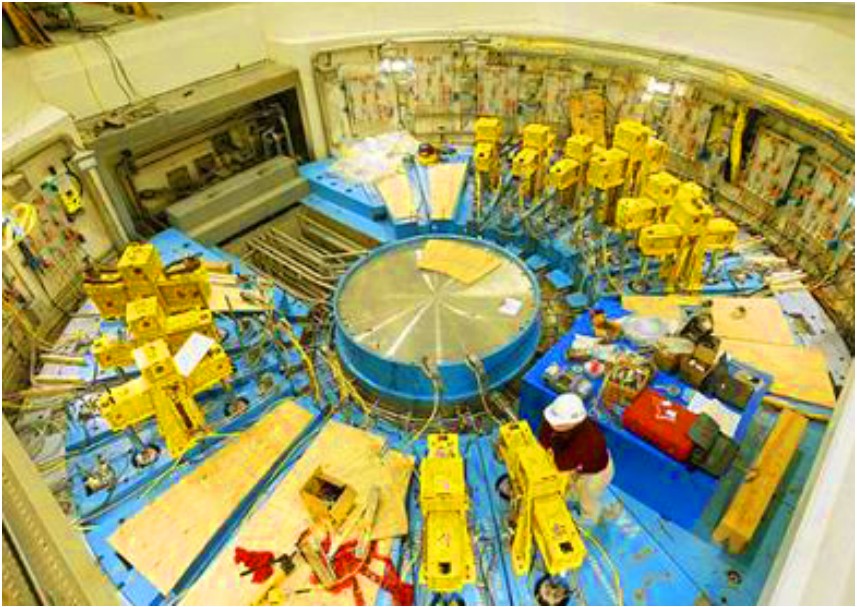
\includegraphics[width=0.27\linewidth]{picture/screenshot070}
\end{figure}



\fourchoices
{${ }_{7}^{14} \mathrm{N}$ 俘获一个 $\alpha$ 粒子,产生 ${ }_{8}^{17} \mathrm{O}$ 并放出一个粒子}
{$27 \mathrm{Al}$ 俘获一个 $\alpha$ 粒子, 产生 ${ }_{15}^{30} \mathrm{P}$ 并放出一个粒子}
{${ }_{5}^{11} \mathrm{B}$ 俘获一个质子,产生 ${ }_{4}^{8} \mathrm{Be}$ 并放出一个粒子}
{${ }_{3}^{6} \mathrm{Li}$ 俘获一个质子,产生 ${ }_{2}^{3} \mathrm{He}$ 并放出一个粒子}


\item 
\exwhere{$ 2018 $ 年全国\lmd{3}卷}
$ 1934 $ 年,约里奥$ - $居里夫妇用 $ \alpha $ 粒子轰击铝核 \ce{^{27}_{13}Al} ,产生了第一个人工
放射性核素 $ X $:$\alpha+{ }_{13}^{27} \mathrm{Al} \rightarrow \mathrm{n}+\mathrm{X}$。$ X $ 的原子序数和质量数分别为 \xzanswer{B} 

\fourchoices
{$ 15 $ 和 $ 28 $}
{$ 15 $ 和 $ 30 $}
{$ 16 $ 和 $ 30 $}
{$ 17 $ 和 $ 31 $}


\item 
\exwhere{$ 2018 $ 年浙江卷($ 4 $ 月选考)}
下列说法正确的是 \xzanswer{BD} 

\fourchoices
{组成原子核的核子越多,原子核越稳定}
{\ce{^{238}_{92}U} 衰变为 \ce{^{222}_{86}Rn} 经过 $ 4 $ 次$ \alpha $衰,$ 2 $ 次$ \beta $衰变}
{在 $ LC $ 振荡电路中,当电流最大时,线圈两端电势差也最大}
{在电子的单缝衍射实验中,狭缝变窄,电子动量的不确定量变大}





	
	
	
\end{enumerate}

